\section[SDD]{Spec-Driven Development}

\begin{frame}
    \frametitle{Vibe coding vs. Spec-Driven Development}
    \begin{columns}[T]
        \begin{column}{0.48\textwidth}
            \begin{block}{Vibe coding}
                \begin{itemize}
                    \item El prompt es efímero
                    \item El código es la única fuente de verdad
                    \item El contexto se pierde entre sesiones
                \end{itemize}
            \end{block}
        \end{column}
        \begin{column}{0.48\textwidth}
            \begin{exampleblock}{SDD}
                \begin{itemize}
                    \item La especificación es la fuente de verdad
                    \item Requisitos, plan y tareas versionados
                    \item Cada artefacto trazable al siguiente
                \end{itemize}
            \end{exampleblock}
        \end{column}
    \end{columns}
\end{frame}

\begin{frame}
    \frametitle{El flujo de Spec Kit~\cite{SpecKit}}
    \begin{center}
        % Generated from img/flujo.mmd by the Makefile
        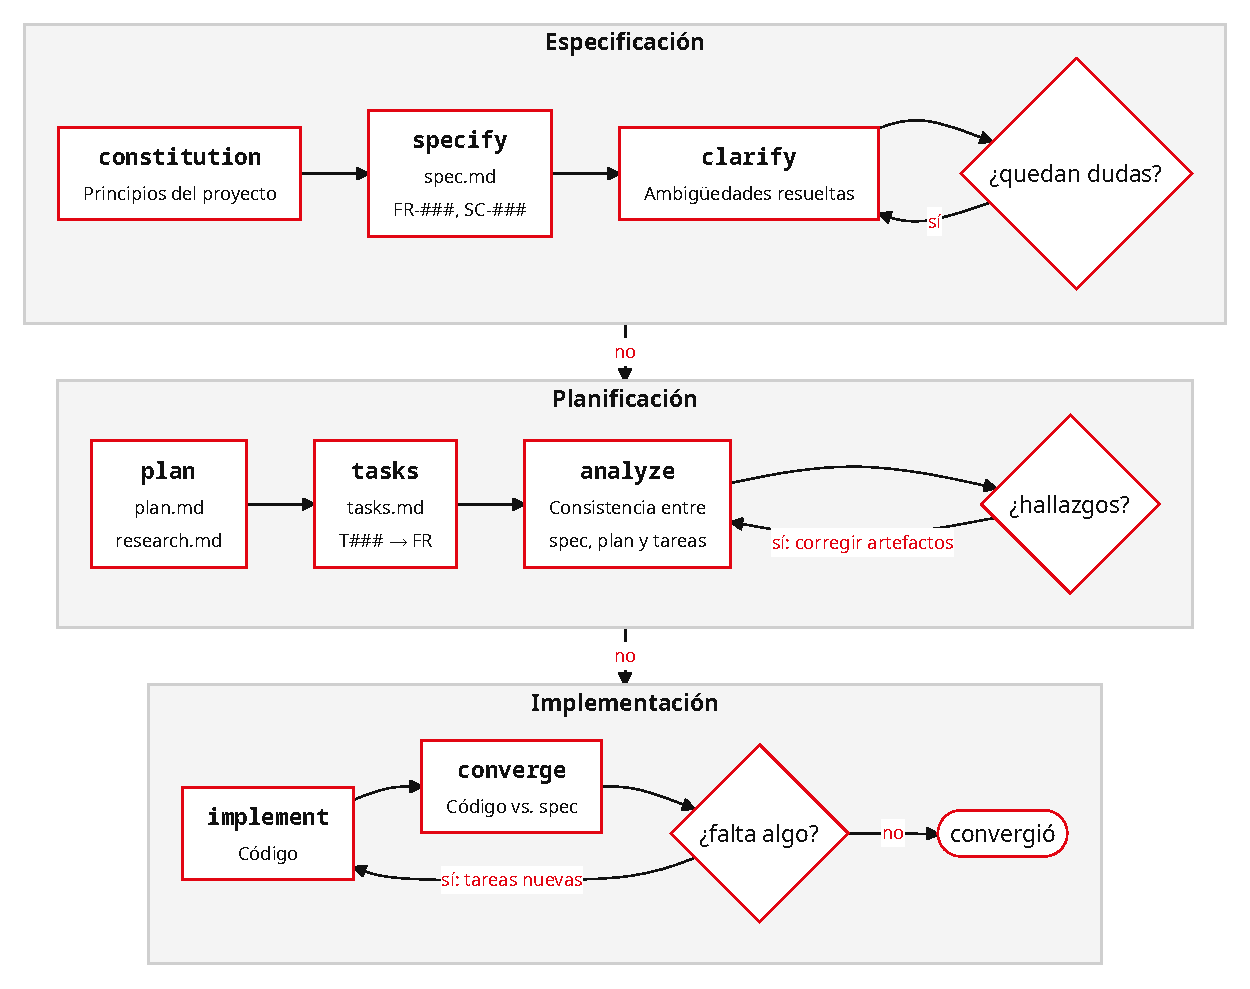
\includegraphics[width=\linewidth,height=4.7cm,keepaspectratio]{img/flujo.pdf}
    \end{center}
\end{frame}

\begin{frame}
    \frametitle{Panorama de implementaciones~\cite{Fowler2025SDD}}
    \begin{itemize}
        \item \textbf{Spec Kit}~\cite{SpecKit}: formal, con fases y trazabilidad explícitas; ideal para proyectos nuevos
        \item \textbf{OpenSpec}~\cite{OpenSpec}: cambios incrementales sobre specs existentes; ideal para proyectos legacy
        \item \textbf{Kiro}~\cite{Kiro}: IDE con requisitos, diseño y tareas integrados
    \end{itemize}
    \begin{alertblock}{Hoy}
        Proyecto nuevo $\Rightarrow$ Spec Kit
    \end{alertblock}
\end{frame}
